% Generated by code/needham.py -- do not edit by hand.
\definecolor{qocA}{rgb}{0.00,0.45,0.70}
\definecolor{qocB}{rgb}{0.90,0.60,0.00}
\definecolor{qocC}{rgb}{0.00,0.62,0.45}
\definecolor{qocD}{rgb}{0.80,0.40,0.00}
\definecolor{qocE}{rgb}{0.80,0.60,0.70}
\definecolor{qocF}{rgb}{0.35,0.70,0.90}
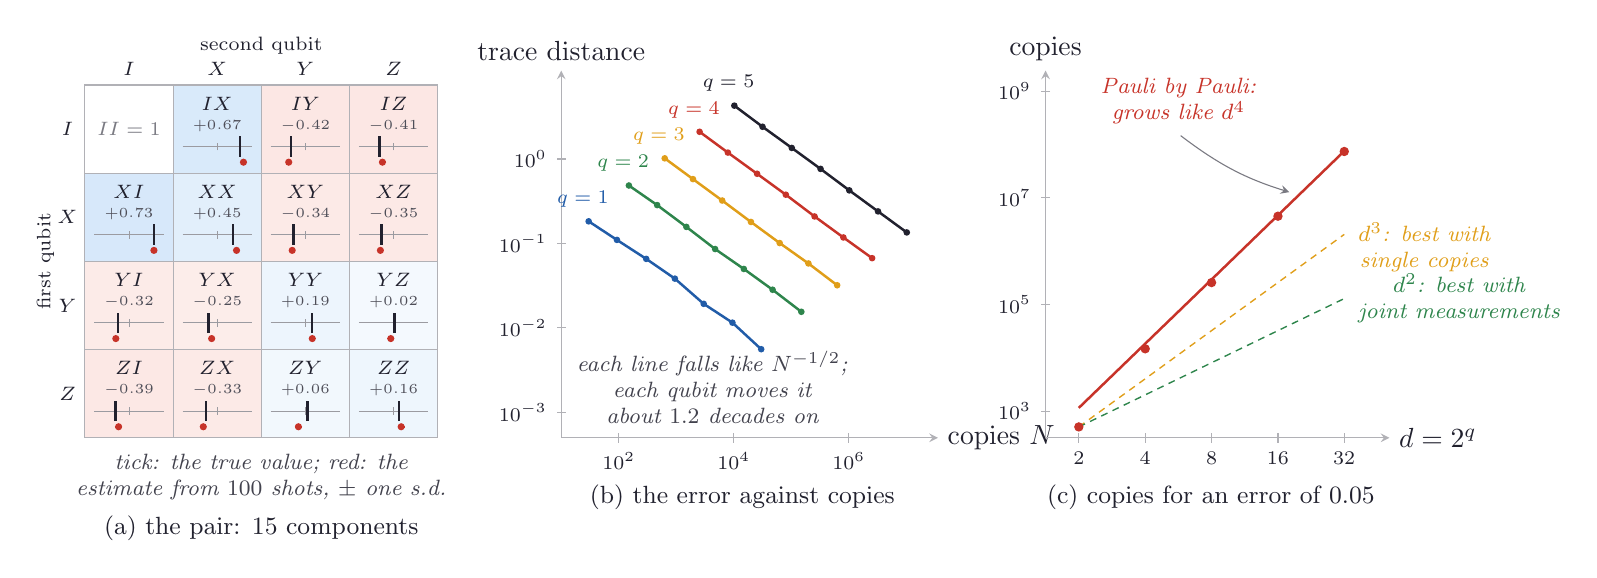
\begin{tikzpicture}[ink/.style={line width=0.9pt, ndInk}, faint/.style={line width=0.4pt, ndInk!35}, dashedink/.style={line width=0.5pt, ndInk!55, dash pattern=on 2.5pt off 2pt}, vec/.style={->, >=stealth, line width=1.2pt}, note/.style={font=\footnotesize\itshape, text=ndInk!85, align=center}, pointer/.style={->, >=stealth, line width=0.4pt, ndInk!60, shorten >=2pt, shorten <=1pt}, dot/.style={circle, fill=ndInk, inner sep=0pt, minimum size=3.4pt}, wash/.style={fill=ndSky, fill opacity=0.55}, every node/.style={text=ndInk}]
\definecolor{ndInk}{rgb}{0.13,0.13,0.18}
\definecolor{ndPaper}{rgb}{0.99,0.96,0.88}
\definecolor{ndSky}{rgb}{0.84,0.91,0.98}
\definecolor{ndRose}{rgb}{0.98,0.86,0.84}
\definecolor{ndBlue}{rgb}{0.13,0.36,0.66}
\definecolor{ndRed}{rgb}{0.78,0.20,0.16}
\definecolor{ndGold}{rgb}{0.88,0.62,0.10}
\definecolor{ndGreen}{rgb}{0.18,0.52,0.30}
\draw[faint] (0.550,3.360) rectangle (1.670,4.480);
\node[font=\scriptsize, text=ndInk!60] at (1.110,3.920) {$II=1$};
\fill[ndSky, fill opacity=0.92] (1.670,3.360) rectangle (2.790,4.480);
\draw[faint] (1.670,3.360) rectangle (2.790,4.480);
\node[font=\scriptsize, anchor=north] at (2.230,4.450) {$IX$};
\draw[line width=0.3pt, ndInk!45] (1.790,3.700) -- (2.670,3.700);
\draw[line width=0.3pt, ndInk!45] (2.230,3.650) -- (2.230,3.750);
\draw[line width=0.9pt, ndInk] (2.523,3.570) -- (2.523,3.830);
\draw[line width=0.6pt, ndRed] (2.536,3.500) -- (2.593,3.500);
\fill[ndRed] (2.564,3.500) circle (1.3pt);
\node[font=\tiny, text=ndInk!80] at (2.230,3.960) {$+0.67$};
\fill[ndRose, fill opacity=0.67] (2.790,3.360) rectangle (3.910,4.480);
\draw[faint] (2.790,3.360) rectangle (3.910,4.480);
\node[font=\scriptsize, anchor=north] at (3.350,4.450) {$IY$};
\draw[line width=0.3pt, ndInk!45] (2.910,3.700) -- (3.790,3.700);
\draw[line width=0.3pt, ndInk!45] (3.350,3.650) -- (3.350,3.750);
\draw[line width=0.9pt, ndInk] (3.166,3.570) -- (3.166,3.830);
\draw[line width=0.6pt, ndRed] (3.100,3.500) -- (3.177,3.500);
\fill[ndRed] (3.139,3.500) circle (1.3pt);
\node[font=\tiny, text=ndInk!80] at (3.350,3.960) {$-0.42$};
\fill[ndRose, fill opacity=0.66] (3.910,3.360) rectangle (5.030,4.480);
\draw[faint] (3.910,3.360) rectangle (5.030,4.480);
\node[font=\scriptsize, anchor=north] at (4.470,4.450) {$IZ$};
\draw[line width=0.3pt, ndInk!45] (4.030,3.700) -- (4.910,3.700);
\draw[line width=0.3pt, ndInk!45] (4.470,3.650) -- (4.470,3.750);
\draw[line width=0.9pt, ndInk] (4.292,3.570) -- (4.292,3.830);
\draw[line width=0.6pt, ndRed] (4.288,3.500) -- (4.371,3.500);
\fill[ndRed] (4.329,3.500) circle (1.3pt);
\node[font=\tiny, text=ndInk!80] at (4.470,3.960) {$-0.41$};
\fill[ndSky, fill opacity=0.98] (0.550,2.240) rectangle (1.670,3.360);
\draw[faint] (0.550,2.240) rectangle (1.670,3.360);
\node[font=\scriptsize, anchor=north] at (1.110,3.330) {$XI$};
\draw[line width=0.3pt, ndInk!45] (0.670,2.580) -- (1.550,2.580);
\draw[line width=0.3pt, ndInk!45] (1.110,2.530) -- (1.110,2.630);
\draw[line width=0.9pt, ndInk] (1.431,2.450) -- (1.431,2.710);
\draw[line width=0.6pt, ndRed] (1.396,2.380) -- (1.457,2.380);
\fill[ndRed] (1.427,2.380) circle (1.3pt);
\node[font=\tiny, text=ndInk!80] at (1.110,2.840) {$+0.73$};
\fill[ndSky, fill opacity=0.70] (1.670,2.240) rectangle (2.790,3.360);
\draw[faint] (1.670,2.240) rectangle (2.790,3.360);
\node[font=\scriptsize, anchor=north] at (2.230,3.330) {$XX$};
\draw[line width=0.3pt, ndInk!45] (1.790,2.580) -- (2.670,2.580);
\draw[line width=0.3pt, ndInk!45] (2.230,2.530) -- (2.230,2.630);
\draw[line width=0.9pt, ndInk] (2.428,2.450) -- (2.428,2.710);
\draw[line width=0.6pt, ndRed] (2.440,2.380) -- (2.513,2.380);
\fill[ndRed] (2.476,2.380) circle (1.3pt);
\node[font=\tiny, text=ndInk!80] at (2.230,2.840) {$+0.45$};
\fill[ndRose, fill opacity=0.59] (2.790,2.240) rectangle (3.910,3.360);
\draw[faint] (2.790,2.240) rectangle (3.910,3.360);
\node[font=\scriptsize, anchor=north] at (3.350,3.330) {$XY$};
\draw[line width=0.3pt, ndInk!45] (2.910,2.580) -- (3.790,2.580);
\draw[line width=0.3pt, ndInk!45] (3.350,2.530) -- (3.350,2.630);
\draw[line width=0.9pt, ndInk] (3.200,2.450) -- (3.200,2.710);
\draw[line width=0.6pt, ndRed] (3.142,2.380) -- (3.223,2.380);
\fill[ndRed] (3.183,2.380) circle (1.3pt);
\node[font=\tiny, text=ndInk!80] at (3.350,2.840) {$-0.34$};
\fill[ndRose, fill opacity=0.60] (3.910,2.240) rectangle (5.030,3.360);
\draw[faint] (3.910,2.240) rectangle (5.030,3.360);
\node[font=\scriptsize, anchor=north] at (4.470,3.330) {$XZ$};
\draw[line width=0.3pt, ndInk!45] (4.030,2.580) -- (4.910,2.580);
\draw[line width=0.3pt, ndInk!45] (4.470,2.530) -- (4.470,2.630);
\draw[line width=0.9pt, ndInk] (4.314,2.450) -- (4.314,2.710);
\draw[line width=0.6pt, ndRed] (4.262,2.380) -- (4.343,2.380);
\fill[ndRed] (4.303,2.380) circle (1.3pt);
\node[font=\tiny, text=ndInk!80] at (4.470,2.840) {$-0.35$};
\fill[ndRose, fill opacity=0.57] (0.550,1.120) rectangle (1.670,2.240);
\draw[faint] (0.550,1.120) rectangle (1.670,2.240);
\node[font=\scriptsize, anchor=north] at (1.110,2.210) {$YI$};
\draw[line width=0.3pt, ndInk!45] (0.670,1.460) -- (1.550,1.460);
\draw[line width=0.3pt, ndInk!45] (1.110,1.410) -- (1.110,1.510);
\draw[line width=0.9pt, ndInk] (0.970,1.330) -- (0.970,1.590);
\draw[line width=0.6pt, ndRed] (0.902,1.260) -- (0.983,1.260);
\fill[ndRed] (0.943,1.260) circle (1.3pt);
\node[font=\tiny, text=ndInk!80] at (1.110,1.720) {$-0.32$};
\fill[ndRose, fill opacity=0.50] (1.670,1.120) rectangle (2.790,2.240);
\draw[faint] (1.670,1.120) rectangle (2.790,2.240);
\node[font=\scriptsize, anchor=north] at (2.230,2.210) {$YX$};
\draw[line width=0.3pt, ndInk!45] (1.790,1.460) -- (2.670,1.460);
\draw[line width=0.3pt, ndInk!45] (2.230,1.410) -- (2.230,1.510);
\draw[line width=0.9pt, ndInk] (2.121,1.330) -- (2.121,1.590);
\draw[line width=0.6pt, ndRed] (2.116,1.260) -- (2.203,1.260);
\fill[ndRed] (2.160,1.260) circle (1.3pt);
\node[font=\tiny, text=ndInk!80] at (2.230,1.720) {$-0.25$};
\fill[ndSky, fill opacity=0.44] (2.790,1.120) rectangle (3.910,2.240);
\draw[faint] (2.790,1.120) rectangle (3.910,2.240);
\node[font=\scriptsize, anchor=north] at (3.350,2.210) {$YY$};
\draw[line width=0.3pt, ndInk!45] (2.910,1.460) -- (3.790,1.460);
\draw[line width=0.3pt, ndInk!45] (3.350,1.410) -- (3.350,1.510);
\draw[line width=0.9pt, ndInk] (3.432,1.330) -- (3.432,1.590);
\draw[line width=0.6pt, ndRed] (3.395,1.260) -- (3.481,1.260);
\fill[ndRed] (3.438,1.260) circle (1.3pt);
\node[font=\tiny, text=ndInk!80] at (3.350,1.720) {$+0.19$};
\fill[ndSky, fill opacity=0.27] (3.910,1.120) rectangle (5.030,2.240);
\draw[faint] (3.910,1.120) rectangle (5.030,2.240);
\node[font=\scriptsize, anchor=north] at (4.470,2.210) {$YZ$};
\draw[line width=0.3pt, ndInk!45] (4.030,1.460) -- (4.910,1.460);
\draw[line width=0.3pt, ndInk!45] (4.470,1.410) -- (4.470,1.510);
\draw[line width=0.9pt, ndInk] (4.480,1.330) -- (4.480,1.590);
\draw[line width=0.6pt, ndRed] (4.391,1.260) -- (4.479,1.260);
\fill[ndRed] (4.435,1.260) circle (1.3pt);
\node[font=\tiny, text=ndInk!80] at (4.470,1.720) {$+0.02$};
\fill[ndRose, fill opacity=0.64] (0.550,0.000) rectangle (1.670,1.120);
\draw[faint] (0.550,0.000) rectangle (1.670,1.120);
\node[font=\scriptsize, anchor=north] at (1.110,1.090) {$ZI$};
\draw[line width=0.3pt, ndInk!45] (0.670,0.340) -- (1.550,0.340);
\draw[line width=0.3pt, ndInk!45] (1.110,0.290) -- (1.110,0.390);
\draw[line width=0.9pt, ndInk] (0.940,0.210) -- (0.940,0.470);
\draw[line width=0.6pt, ndRed] (0.936,0.140) -- (1.020,0.140);
\fill[ndRed] (0.978,0.140) circle (1.3pt);
\node[font=\tiny, text=ndInk!80] at (1.110,0.600) {$-0.39$};
\fill[ndRose, fill opacity=0.58] (1.670,0.000) rectangle (2.790,1.120);
\draw[faint] (1.670,0.000) rectangle (2.790,1.120);
\node[font=\scriptsize, anchor=north] at (2.230,1.090) {$ZX$};
\draw[line width=0.3pt, ndInk!45] (1.790,0.340) -- (2.670,0.340);
\draw[line width=0.3pt, ndInk!45] (2.230,0.290) -- (2.230,0.390);
\draw[line width=0.9pt, ndInk] (2.086,0.210) -- (2.086,0.470);
\draw[line width=0.6pt, ndRed] (2.014,0.140) -- (2.094,0.140);
\fill[ndRed] (2.054,0.140) circle (1.3pt);
\node[font=\tiny, text=ndInk!80] at (2.230,0.600) {$-0.33$};
\fill[ndSky, fill opacity=0.31] (2.790,0.000) rectangle (3.910,1.120);
\draw[faint] (2.790,0.000) rectangle (3.910,1.120);
\node[font=\scriptsize, anchor=north] at (3.350,1.090) {$ZY$};
\draw[line width=0.3pt, ndInk!45] (2.910,0.340) -- (3.790,0.340);
\draw[line width=0.3pt, ndInk!45] (3.350,0.290) -- (3.350,0.390);
\draw[line width=0.9pt, ndInk] (3.378,0.210) -- (3.378,0.470);
\draw[line width=0.6pt, ndRed] (3.219,0.140) -- (3.305,0.140);
\fill[ndRed] (3.262,0.140) circle (1.3pt);
\node[font=\tiny, text=ndInk!80] at (3.350,0.600) {$+0.06$};
\fill[ndSky, fill opacity=0.41] (3.910,0.000) rectangle (5.030,1.120);
\draw[faint] (3.910,0.000) rectangle (5.030,1.120);
\node[font=\scriptsize, anchor=north] at (4.470,1.090) {$ZZ$};
\draw[line width=0.3pt, ndInk!45] (4.030,0.340) -- (4.910,0.340);
\draw[line width=0.3pt, ndInk!45] (4.470,0.290) -- (4.470,0.390);
\draw[line width=0.9pt, ndInk] (4.539,0.210) -- (4.539,0.470);
\draw[line width=0.6pt, ndRed] (4.524,0.140) -- (4.610,0.140);
\fill[ndRed] (4.567,0.140) circle (1.3pt);
\node[font=\tiny, text=ndInk!80] at (4.470,0.600) {$+0.16$};
\node[font=\scriptsize] at (0.330,3.920) {$I$};
\node[font=\scriptsize] at (1.110,4.680) {$I$};
\node[font=\scriptsize] at (0.330,2.800) {$X$};
\node[font=\scriptsize] at (2.230,4.680) {$X$};
\node[font=\scriptsize] at (0.330,1.680) {$Y$};
\node[font=\scriptsize] at (3.350,4.680) {$Y$};
\node[font=\scriptsize] at (0.330,0.560) {$Z$};
\node[font=\scriptsize] at (4.470,4.680) {$Z$};
\node[font=\scriptsize, rotate=90] at (0.050,2.240) {first qubit};
\node[font=\scriptsize] at (2.790,4.980) {second qubit};
\node[note, anchor=north] at (2.79,-0.08) {tick: the true value; red: the\\ estimate from $100$ shots, $\pm$ one s.d.};
\node[font=\small] at (2.79,-1.15) {(a) the pair: $15$ components};
\draw[faint, ->, >=stealth] (6.600,0.000) -- (11.384,0.000) node[right, text=ndInk] {copies $N$};
\draw[faint, ->, >=stealth] (6.600,0.000) -- (6.600,4.664) node[above, text=ndInk] {trace distance};
\draw[faint] (7.330,0.060) -- (7.330,-0.060) node[below, font=\scriptsize, text=ndInk] {$10^{2}$};
\draw[faint] (8.790,0.060) -- (8.790,-0.060) node[below, font=\scriptsize, text=ndInk] {$10^{4}$};
\draw[faint] (10.251,0.060) -- (10.251,-0.060) node[below, font=\scriptsize, text=ndInk] {$10^{6}$};
\draw[faint] (6.660,0.322) -- (6.540,0.322) node[left, font=\scriptsize, text=ndInk] {$10^{-3}$};
\draw[faint] (6.660,1.395) -- (6.540,1.395) node[left, font=\scriptsize, text=ndInk] {$10^{-2}$};
\draw[faint] (6.660,2.468) -- (6.540,2.468) node[left, font=\scriptsize, text=ndInk] {$10^{-1}$};
\draw[faint] (6.660,3.541) -- (6.540,3.541) node[left, font=\scriptsize, text=ndInk] {$10^{0}$};
\draw[line width=0.9pt, ndBlue] (6.948,2.749) -- (7.307,2.513) -- (7.679,2.272) -- (8.043,2.021) -- (8.409,1.701) -- (8.774,1.462) -- (9.139,1.125);
\fill[ndBlue] (6.948,2.749) circle (1.2pt);
\fill[ndBlue] (7.307,2.513) circle (1.2pt);
\fill[ndBlue] (7.679,2.272) circle (1.2pt);
\fill[ndBlue] (8.043,2.021) circle (1.2pt);
\fill[ndBlue] (8.409,1.701) circle (1.2pt);
\fill[ndBlue] (8.774,1.462) circle (1.2pt);
\fill[ndBlue] (9.139,1.125) circle (1.2pt);
\node[font=\scriptsize, text=ndBlue, anchor=south] at (6.875,2.803) {$q=1$};
\draw[line width=0.9pt, ndGreen] (7.459,3.204) -- (7.818,2.955) -- (8.189,2.678) -- (8.554,2.397) -- (8.919,2.144) -- (9.284,1.880) -- (9.649,1.600);
\fill[ndGreen] (7.459,3.204) circle (1.2pt);
\fill[ndGreen] (7.818,2.955) circle (1.2pt);
\fill[ndGreen] (8.189,2.678) circle (1.2pt);
\fill[ndGreen] (8.554,2.397) circle (1.2pt);
\fill[ndGreen] (8.919,2.144) circle (1.2pt);
\fill[ndGreen] (9.284,1.880) circle (1.2pt);
\fill[ndGreen] (9.649,1.600) circle (1.2pt);
\node[font=\scriptsize, text=ndGreen, anchor=south] at (7.386,3.258) {$q=2$};
\draw[line width=0.9pt, ndGold] (7.914,3.549) -- (8.273,3.285) -- (8.644,3.013) -- (9.009,2.741) -- (9.374,2.473) -- (9.739,2.214) -- (10.104,1.937);
\fill[ndGold] (7.914,3.549) circle (1.2pt);
\fill[ndGold] (8.273,3.285) circle (1.2pt);
\fill[ndGold] (8.644,3.013) circle (1.2pt);
\fill[ndGold] (9.009,2.741) circle (1.2pt);
\fill[ndGold] (9.374,2.473) circle (1.2pt);
\fill[ndGold] (9.739,2.214) circle (1.2pt);
\fill[ndGold] (10.104,1.937) circle (1.2pt);
\node[font=\scriptsize, text=ndGold, anchor=south] at (7.841,3.603) {$q=3$};
\draw[line width=0.9pt, ndRed] (8.357,3.886) -- (8.716,3.622) -- (9.087,3.353) -- (9.452,3.087) -- (9.817,2.811) -- (10.183,2.544) -- (10.548,2.281);
\fill[ndRed] (8.357,3.886) circle (1.2pt);
\fill[ndRed] (8.716,3.622) circle (1.2pt);
\fill[ndRed] (9.087,3.353) circle (1.2pt);
\fill[ndRed] (9.452,3.087) circle (1.2pt);
\fill[ndRed] (9.817,2.811) circle (1.2pt);
\fill[ndRed] (10.183,2.544) circle (1.2pt);
\fill[ndRed] (10.548,2.281) circle (1.2pt);
\node[font=\scriptsize, text=ndRed, anchor=south] at (8.284,3.940) {$q=4$};
\draw[line width=0.9pt, ndInk] (8.798,4.218) -- (9.156,3.950) -- (9.528,3.681) -- (9.893,3.415) -- (10.258,3.142) -- (10.623,2.875) -- (10.988,2.608);
\fill[ndInk] (8.798,4.218) circle (1.2pt);
\fill[ndInk] (9.156,3.950) circle (1.2pt);
\fill[ndInk] (9.528,3.681) circle (1.2pt);
\fill[ndInk] (9.893,3.415) circle (1.2pt);
\fill[ndInk] (10.258,3.142) circle (1.2pt);
\fill[ndInk] (10.623,2.875) circle (1.2pt);
\fill[ndInk] (10.988,2.608) circle (1.2pt);
\node[font=\scriptsize, text=ndInk, anchor=south] at (8.725,4.272) {$q=5$};
\node[note, anchor=south west] at (6.673,0.054) {each line falls like $N^{-1/2}$;\\ each qubit moves it\\ about $1.2$ decades on};
\node[font=\small] at (8.900,-0.750) {(b) the error against copies};
\draw[faint, ->, >=stealth] (12.750,0.000) -- (17.118,0.000) node[right, text=ndInk] {$d=2^q$};
\draw[faint, ->, >=stealth] (12.750,0.000) -- (12.750,4.664) node[above, text=ndInk] {copies};
\draw[faint] (13.173,0.060) -- (13.173,-0.060) node[below, font=\scriptsize, text=ndInk] {$2$};
\draw[faint] (14.016,0.060) -- (14.016,-0.060) node[below, font=\scriptsize, text=ndInk] {$4$};
\draw[faint] (14.859,0.060) -- (14.859,-0.060) node[below, font=\scriptsize, text=ndInk] {$8$};
\draw[faint] (15.702,0.060) -- (15.702,-0.060) node[below, font=\scriptsize, text=ndInk] {$16$};
\draw[faint] (16.544,0.060) -- (16.544,-0.060) node[below, font=\scriptsize, text=ndInk] {$32$};
\draw[faint] (12.810,0.338) -- (12.690,0.338) node[left, font=\scriptsize, text=ndInk] {$10^{3}$};
\draw[faint] (12.810,1.692) -- (12.690,1.692) node[left, font=\scriptsize, text=ndInk] {$10^{5}$};
\draw[faint] (12.810,3.046) -- (12.690,3.046) node[left, font=\scriptsize, text=ndInk] {$10^{7}$};
\draw[faint] (12.810,4.400) -- (12.690,4.400) node[left, font=\scriptsize, text=ndInk] {$10^{9}$};
\draw[dashedink, ndGold] (13.173,0.138) -- (14.016,0.749) -- (14.859,1.361) -- (15.702,1.972) -- (16.544,2.583);
\node[note, text=ndGold, anchor=west] at (16.600,2.414) {$d^3$: best with\\ single copies};
\draw[dashedink, ndGreen] (13.173,0.138) -- (14.016,0.545) -- (14.859,0.953) -- (15.702,1.361) -- (16.544,1.768);
\node[note, text=ndGreen, anchor=west] at (16.600,1.768) {$d^2$: best with\\ joint measurements};
\draw[line width=0.9pt, ndRed] (13.173,0.380) -- (14.016,1.195) -- (14.859,2.010) -- (15.702,2.826) -- (16.544,3.641);
\node[dot, fill=ndRed] at (13.173,0.138) {};
\node[dot, fill=ndRed] at (14.016,1.130) {};
\node[dot, fill=ndRed] at (14.859,1.971) {};
\node[dot, fill=ndRed] at (15.702,2.814) {};
\node[dot, fill=ndRed] at (16.544,3.636) {};
\node[note, text=ndRed, anchor=south east] (f) at (15.550,3.858) {Pauli by Pauli:\\ grows like $d^4$};
\draw[pointer] (f.south) to[bend right=10] (15.914,3.099);
\node[font=\small] at (14.850,-0.750) {(c) copies for an error of $0.05$};
\end{tikzpicture}
